\chapter{Test Domain Models}

We used two domain models to test the Service Cutter. Both domain models are presented in this chapter.

\section{Trading System}

The Trading System was developed by us and its goal is to include various different coupling aspects in a rather small domain model.

The Trading System is an application one might find in a typical swiss private bank offering its customers the ability to manage their stocks portfolio.

\begin{itemize}
\item The main focus is to buy or sell \textit{stocks} at a specific price (\textit{Order.triggerPrice}) using an \textit{order}.
\item \textit{Prices} are frequently imported from an market data provider and upon import of a price, all orders are checked for orders that can be triggered.
\item When an order is executed, an instruction is sent to the market to purchase or sell the stocks. The \textit{payment info} contains all necessary information to do so. 
\item \textit{News} are imported from an external provider and are linked to a specific stock. They provide valuable, contextual information when using the system. However traders and customers can easily fall back to any online source should this information not be available.
\item \textit{Recommendations} are suggested to the user of the system based on his existing portfolio.
\end{itemize}

Figure \ref{fig:tradingClasses} shows a class diagram of the Trading System.

\begin{figure}[H]
	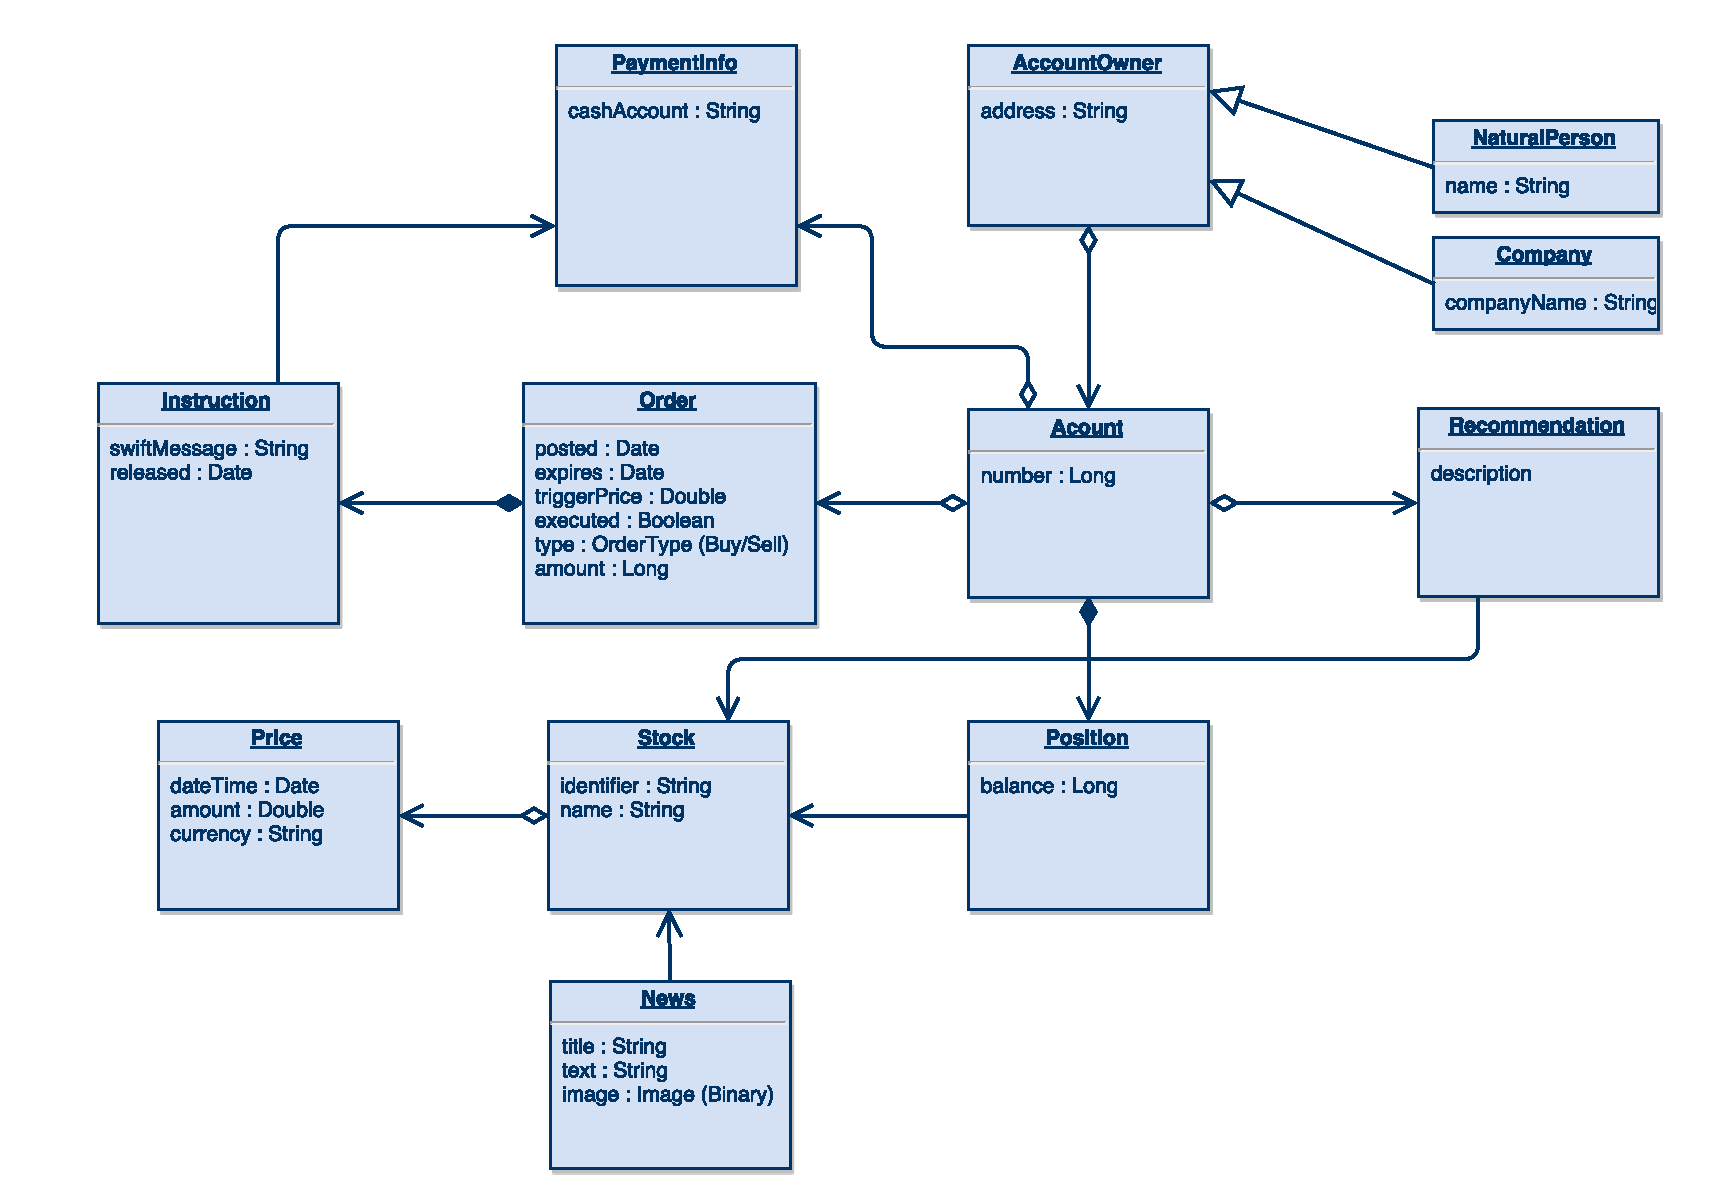
\includegraphics[scale=0.5]{diagrams/TradingSystem.pdf}
	\caption{Trading System Class Diagram}
	\label{fig:tradingClasses}
\end{figure}

The following ten Use Cases describe the supported functionality of the application.

\begin{enumerate}
\item Post Order
	\begin{itemize}
	\item Fields written: Order.posted,  Order.expires, Order.triggerPrice, Order.executed, Order.type, Order.amount
	\item Fields read: Account.number, Stock.identifier, Stock.stockName
	\end{itemize}
\item Instruct Order
	\begin{itemize}
	\item Fields written: Instruction.instructedTime, Order.executed, Position.balance
	\item Fields read: PaymentInfo.cashAccount
	\end{itemize}
\item Import Price and Check for Due Orders (Technical)
	\begin{itemize}
	\item Fields written: Price.dateTime, Price.price, Price.currency
	\item Fields read: Order.triggerPrice, Stock.identifier
	\end{itemize}
\item Read News
	\begin{itemize}
	\item Fields written: - 
	\item Fields read: Stock.identifier, News.title, News.text, News.image
	\end{itemize}
\item Import News (Technical)
	\begin{itemize}
	\item Fields written: News.title, News.text, News.image
	\item Fields read: Stock.identifier
	\end{itemize}
\item View Recommendations
	\begin{itemize}
	\item Fields written: -
	\item Fields read: Account.number, Recommendation.description, Stock.identifier, Stock.stockName
	\end{itemize}
\item Suggest Recommendations (Technical)
	\begin{itemize}
	\item Fields written: Recommendation.description
	\item Fields read: Account.number, Stock.identifier, Stock.stockName, Position.balance
	\end{itemize}
\item Create Account
	\begin{itemize}
	\item Fields written: Account.number
	\item Fields read: AccountOwner.address, NaturalPerson.name, Company.companyName
	\end{itemize}
\item Create Account Owner
	\begin{itemize}
	\item Fields written: AccountOwner.address, NaturalPerson.name, Company.companyName
	\item Fields read: -
	\end{itemize}
\item View Portfolio
	\begin{itemize}
	\item Fields written: -
	\item Fields read: Account.number, Position.balance, Stock.identifier, Stock.stockName, Order.triggerPrice, Order.amount, Order.posted, Order.expires, Order.executed, Order.type
	\end{itemize}
\end{enumerate}

In addition to the use cases, we defined the following characteristics.

\textbf{Security Criticality}

\begin{itemize}
\item \textbf{Public}: Stock.identifier,Stock.stockName, Price.dateTime, Price.price, Price.currency, News.title, News.text, News.image
\item \textbf{Critical}: AccountOwner.address, NaturalPerson.name, Company.companyName
\end{itemize} 

\textbf{Volatility}

\begin{itemize}
\item \textbf{Often}: Price.dateTime, Price.price, Price.currency
\item \textbf{Rarely}: AccountOwner.address, NaturalPerson.name, Company.companyName, Account.number
\end{itemize}

\textbf{Consistency}

\begin{itemize}
\item \textbf{Eventually}: Price.dateTime, Price.price, Price.currency
\end{itemize}

\textbf{Storage Similarity}

\begin{itemize}
\item \textbf{Huge}: News.image
\end{itemize}

\textbf{Change Similarity}

\begin{itemize}
\item \textbf{Often}: Recommendation.description
\end{itemize}

\textbf{Resilience}

\begin{itemize}
\item \textbf{Low}: News.title, News.text, News.image, Recommendation.description
\end{itemize}

Furthermore all default styles of characteristics as documented in Section \ref{sec:couplingCriteria} are taken into account.

From our experience we expect the Service Cutter to decompose the Trading System into the services presented in Figure \ref{fig:tradingCuts}.

\begin{figure}[H]
	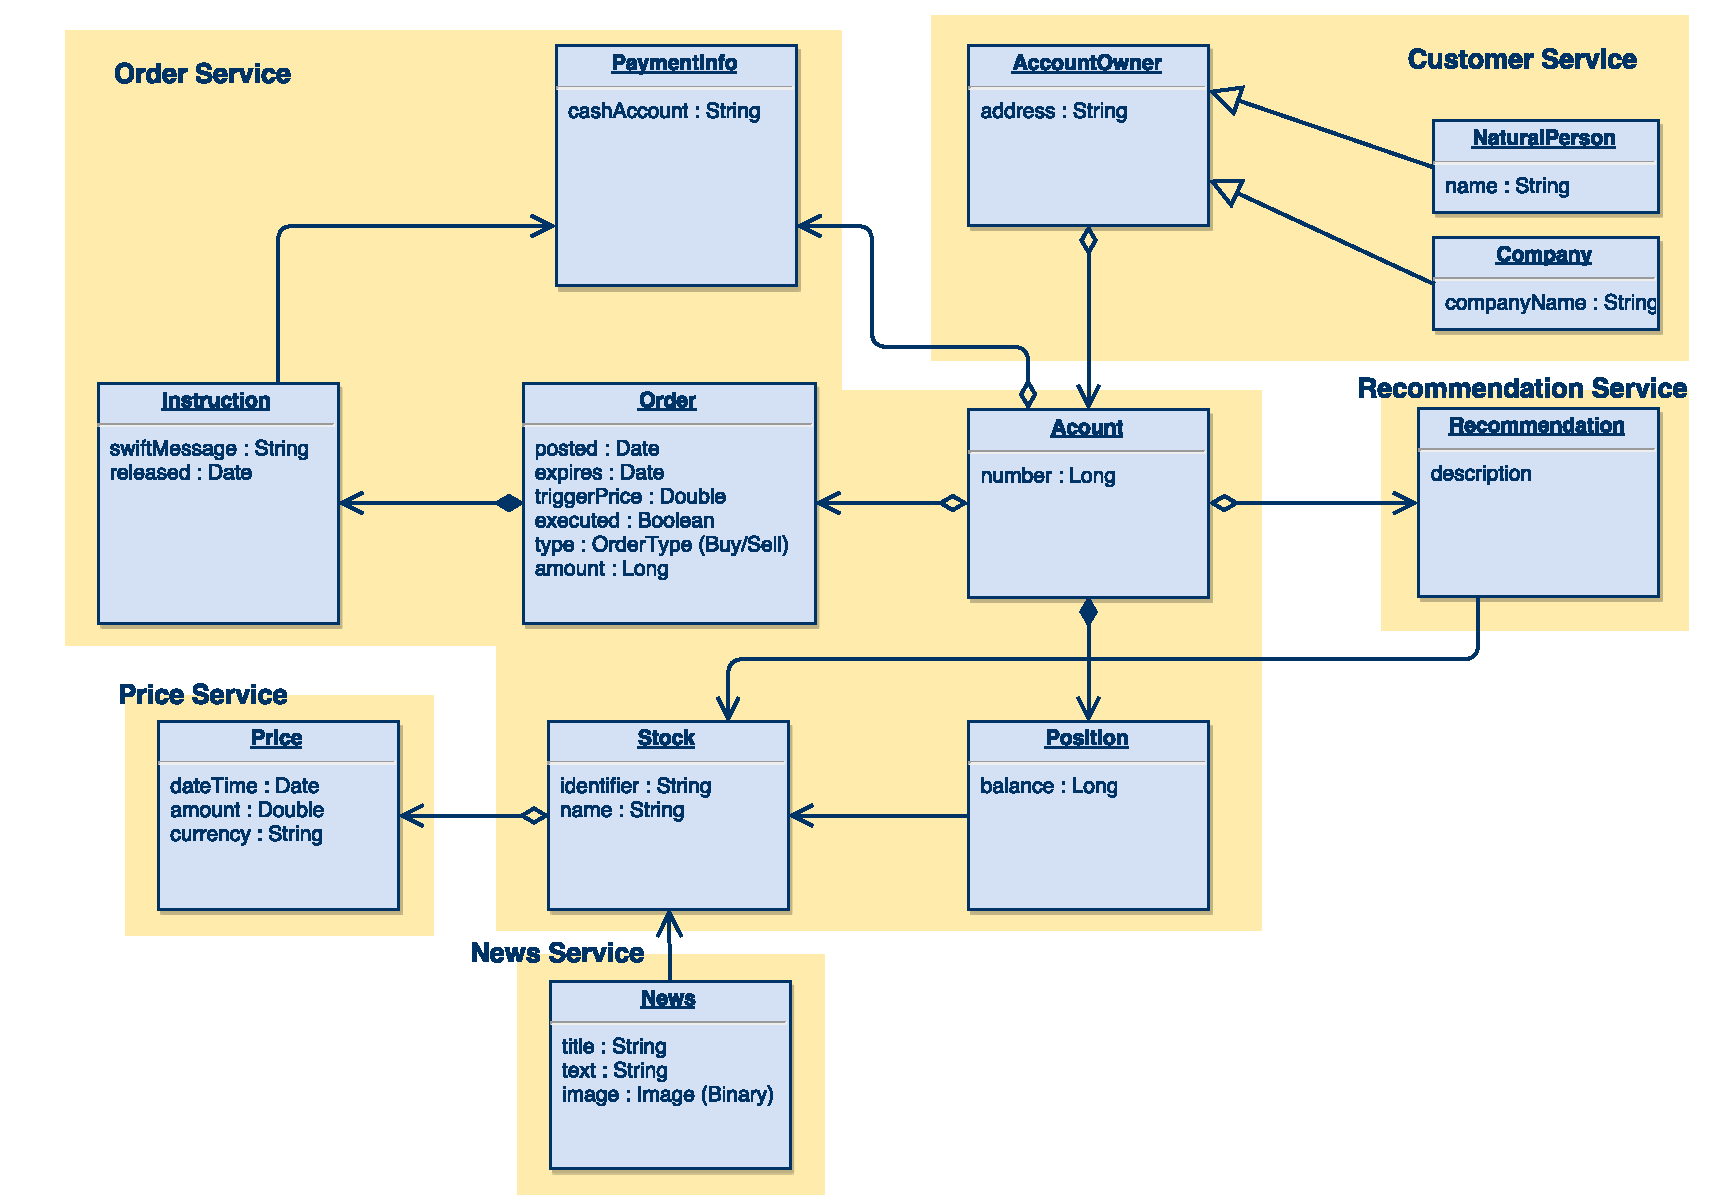
\includegraphics[scale=0.5]{diagrams/TradingSystem-ServiceCut.pdf}
	\caption{Trading System expected service cuts}
	\label{fig:tradingCuts}
\end{figure}

The following reasons led us to this decision.
\begin{itemize}
	\item The service \textit{Order} encapsulated many use cases and contains several entities that need to be processed with high consistency (Order, Position).
	\item The high volatility of the entity price led to the isolation of this part into an own service \textit{Price}.
	\item News images require a significant amount of storage. Therefore we would isolate this into a separate \textit{News} service allowing an optimized storage technology.
	\item The recommendation algorithm will be changed frequently. A dedicated \textit{Recommendation} service allows independent deployment of updated versions.
	\item Security restrictions requires all \gls{PII} to be separated from other data. Extracting it into a \textit{Customer} service allows the architect to protect this data with additional measures.
\end{itemize}

Figure \ref{fig:tradingCutsTool} is the suggested cut as calculated by the Service Cutter. 

\begin{figure}[H]
	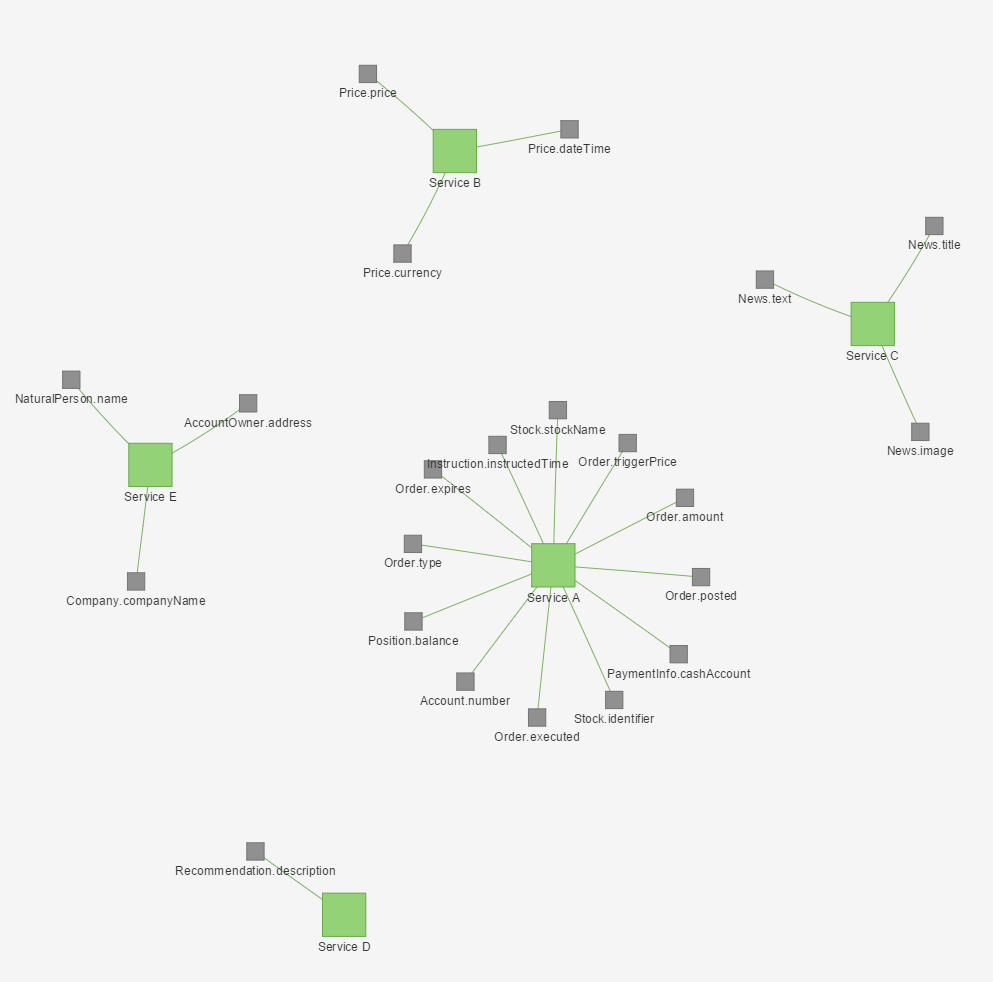
\includegraphics[scale=0.5]{images/trading_service_cut.png}
	\caption{Trading System actual service cuts}
	\label{fig:tradingCutsTool}
\end{figure}

The parameters that produce a cut as seen in \ref{fig:tradingCutsTool} are the following:

\begin{itemize}
\item Coupling Criteria priorities: M for all criteria
\item Algorithm: Girvan-Newman
\item Number of clusters: 5
\end{itemize}

Leung produces varying suggested cuts as it is not a deterministic algorithm. We have observed the following variations:

\begin{enumerate}
\item Account.number, ParmentInfo.cashAccount and Position.balance are separated into a service.
\item PaymentInfo.cashAccount is separated into a service.
\item News are incorporated into the main \textit{Order} service.
\end{enumerate}

However fairly stable results matching the expectations have been tested with the following priorities:

\begin{itemize}
\item Coupling Criteria priorities:
	\begin{itemize}
	\item L for \enquote{Identity \& Lifecycle Commonality} and \enquote{Semantic Proximity}
	\item M for all others
	\end{itemize}
\end{itemize}

In conclusion we can say that the Service Cutter did suggest the Trading System service cuts we expected.